\documentclass{article}\usepackage[]{graphicx}\usepackage[]{color}
%% maxwidth is the original width if it is less than linewidth
%% otherwise use linewidth (to make sure the graphics do not exceed the margin)
\makeatletter
\def\maxwidth{ %
  \ifdim\Gin@nat@width>\linewidth
    \linewidth
  \else
    \Gin@nat@width
  \fi
}
\makeatother

\definecolor{fgcolor}{rgb}{0.345, 0.345, 0.345}
\newcommand{\hlnum}[1]{\textcolor[rgb]{0.686,0.059,0.569}{#1}}%
\newcommand{\hlstr}[1]{\textcolor[rgb]{0.192,0.494,0.8}{#1}}%
\newcommand{\hlcom}[1]{\textcolor[rgb]{0.678,0.584,0.686}{\textit{#1}}}%
\newcommand{\hlopt}[1]{\textcolor[rgb]{0,0,0}{#1}}%
\newcommand{\hlstd}[1]{\textcolor[rgb]{0.345,0.345,0.345}{#1}}%
\newcommand{\hlkwa}[1]{\textcolor[rgb]{0.161,0.373,0.58}{\textbf{#1}}}%
\newcommand{\hlkwb}[1]{\textcolor[rgb]{0.69,0.353,0.396}{#1}}%
\newcommand{\hlkwc}[1]{\textcolor[rgb]{0.333,0.667,0.333}{#1}}%
\newcommand{\hlkwd}[1]{\textcolor[rgb]{0.737,0.353,0.396}{\textbf{#1}}}%

\usepackage{framed}
\makeatletter
\newenvironment{kframe}{%
 \def\at@end@of@kframe{}%
 \ifinner\ifhmode%
  \def\at@end@of@kframe{\end{minipage}}%
  \begin{minipage}{\columnwidth}%
 \fi\fi%
 \def\FrameCommand##1{\hskip\@totalleftmargin \hskip-\fboxsep
 \colorbox{shadecolor}{##1}\hskip-\fboxsep
     % There is no \\@totalrightmargin, so:
     \hskip-\linewidth \hskip-\@totalleftmargin \hskip\columnwidth}%
 \MakeFramed {\advance\hsize-\width
   \@totalleftmargin\z@ \linewidth\hsize
   \@setminipage}}%
 {\par\unskip\endMakeFramed%
 \at@end@of@kframe}
\makeatother

\definecolor{shadecolor}{rgb}{.97, .97, .97}
\definecolor{messagecolor}{rgb}{0, 0, 0}
\definecolor{warningcolor}{rgb}{1, 0, 1}
\definecolor{errorcolor}{rgb}{1, 0, 0}
\newenvironment{knitrout}{}{} % an empty environment to be redefined in TeX

\usepackage{alltt}
\usepackage{geometry}
\usepackage{graphicx}
\usepackage[lofdepth,lotdepth]{subfig}
\title{KnitR tutorial}
\author{Thomas D. Als}
\IfFileExists{upquote.sty}{\usepackage{upquote}}{}
\begin{document}
\maketitle

Loading packages and data:
\begin{knitrout}
\definecolor{shadecolor}{rgb}{0.969, 0.969, 0.969}\color{fgcolor}\begin{kframe}
\begin{alltt}
\hlkwd{setwd}\hlstd{(}\hlstr{"/Users/tdas/Documents/R/ReproducibleResearch_and_DataVisualisation_in_R/RepResDatViz_ALS/StudentMaterials/turtorailKnitr_ALS"}\hlstd{)}
\hlkwd{library}\hlstd{(ggplot2)}
\hlkwd{data}\hlstd{(mpg)}
\end{alltt}
\end{kframe}
\end{knitrout}

Explore data
\begin{knitrout}
\definecolor{shadecolor}{rgb}{0.969, 0.969, 0.969}\color{fgcolor}\begin{kframe}
\begin{alltt}
\hlkwd{head}\hlstd{(mpg)}
\end{alltt}
\begin{verbatim}
##   manufacturer model displ year cyl      trans drv cty hwy fl   class
## 1         audi    a4   1.8 1999   4   auto(l5)   f  18  29  p compact
## 2         audi    a4   1.8 1999   4 manual(m5)   f  21  29  p compact
## 3         audi    a4   2.0 2008   4 manual(m6)   f  20  31  p compact
## 4         audi    a4   2.0 2008   4   auto(av)   f  21  30  p compact
## 5         audi    a4   2.8 1999   6   auto(l5)   f  16  26  p compact
## 6         audi    a4   2.8 1999   6 manual(m5)   f  18  26  p compact
\end{verbatim}
\begin{alltt}
\hlkwd{str}\hlstd{(mpg)}
\end{alltt}
\begin{verbatim}
## 'data.frame':	234 obs. of  11 variables:
##  $ manufacturer: Factor w/ 15 levels "audi","chevrolet",..: 1 1 1 1 1 1 1 1 1 1 ...
##  $ model       : Factor w/ 38 levels "4runner 4wd",..: 2 2 2 2 2 2 2 3 3 3 ...
##  $ displ       : num  1.8 1.8 2 2 2.8 2.8 3.1 1.8 1.8 2 ...
##  $ year        : int  1999 1999 2008 2008 1999 1999 2008 1999 1999 2008 ...
##  $ cyl         : int  4 4 4 4 6 6 6 4 4 4 ...
##  $ trans       : Factor w/ 10 levels "auto(av)","auto(l3)",..: 4 9 10 1 4 9 1 9 4 10 ...
##  $ drv         : Factor w/ 3 levels "4","f","r": 2 2 2 2 2 2 2 1 1 1 ...
##  $ cty         : int  18 21 20 21 16 18 18 18 16 20 ...
##  $ hwy         : int  29 29 31 30 26 26 27 26 25 28 ...
##  $ fl          : Factor w/ 5 levels "c","d","e","p",..: 4 4 4 4 4 4 4 4 4 4 ...
##  $ class       : Factor w/ 7 levels "2seater","compact",..: 2 2 2 2 2 2 2 2 2 2 ...
\end{verbatim}
\end{kframe}
\end{knitrout}

\begin{knitrout}
\definecolor{shadecolor}{rgb}{0.969, 0.969, 0.969}\color{fgcolor}\begin{kframe}
\begin{alltt}
\hlkwd{pairs}\hlstd{(mpg)}
\end{alltt}
\end{kframe}\begin{figure}
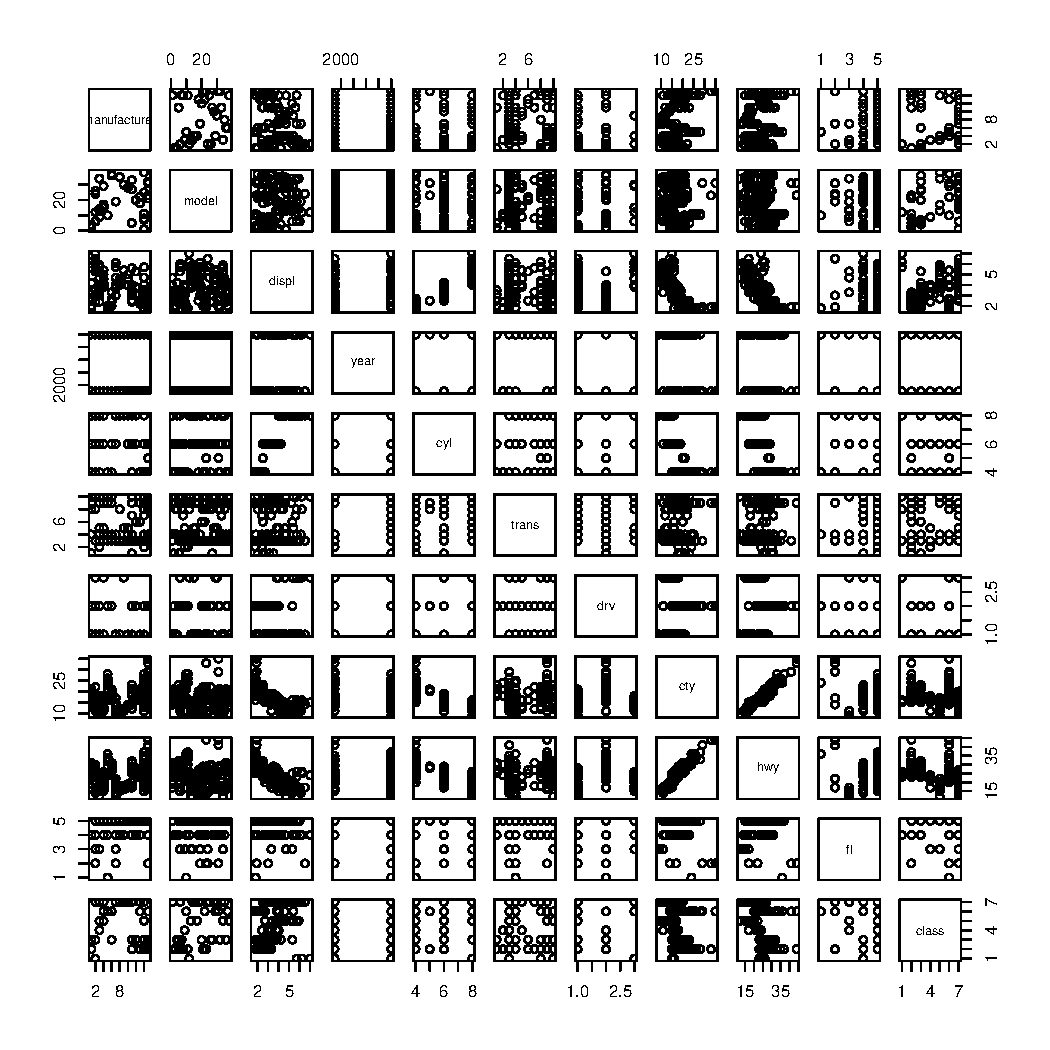
\includegraphics[width=\maxwidth]{figure/plot01-1} \caption[Figure 1]{Figure 1: pairs plot of all variables}\label{fig:plot01}
\end{figure}


\end{knitrout}


Initial plot of the following variables:
displ = engine displacement, in litres
cty = city miles per gallon
model = model
drv = f = fron wheel, r = rear wheel, 4 = four wheel
\begin{knitrout}
\definecolor{shadecolor}{rgb}{0.969, 0.969, 0.969}\color{fgcolor}\begin{kframe}
\begin{alltt}
\hlkwd{ggplot}\hlstd{(mpg,}\hlkwd{aes}\hlstd{(}\hlkwc{x}\hlstd{=displ,}\hlkwc{y}\hlstd{=cty,}\hlkwc{fill}\hlstd{=drv))}\hlopt{+}\hlkwd{geom_point}\hlstd{(}\hlkwc{stat}\hlstd{=}\hlstr{"identity"}\hlstd{,}\hlkwc{position}\hlstd{=}\hlstr{"identity"}\hlstd{)}\hlopt{+}\hlkwd{geom_smooth}\hlstd{(}\hlkwc{size}\hlstd{=}\hlnum{1}\hlstd{)}\hlopt{+}\hlkwd{scale_color_hue}\hlstd{(}\hlstr{"Drive:"}\hlstd{,} \hlkwc{breaks}\hlstd{=}\hlkwd{c}\hlstd{(}\hlnum{1}\hlstd{,}\hlnum{2}\hlstd{,}\hlnum{3}\hlstd{),}\hlkwc{labels}\hlstd{=}\hlkwd{c}\hlstd{(}\hlstr{"4wd"}\hlstd{,}\hlstr{"front"}\hlstd{,}\hlstr{"rear"}\hlstd{))}
\end{alltt}


{\ttfamily\noindent\itshape\color{messagecolor}{\#\# geom\_smooth: method="{}auto"{} and size of largest group is <1000, so using loess. Use 'method = x' to change the smoothing method.}}\end{kframe}\begin{figure}
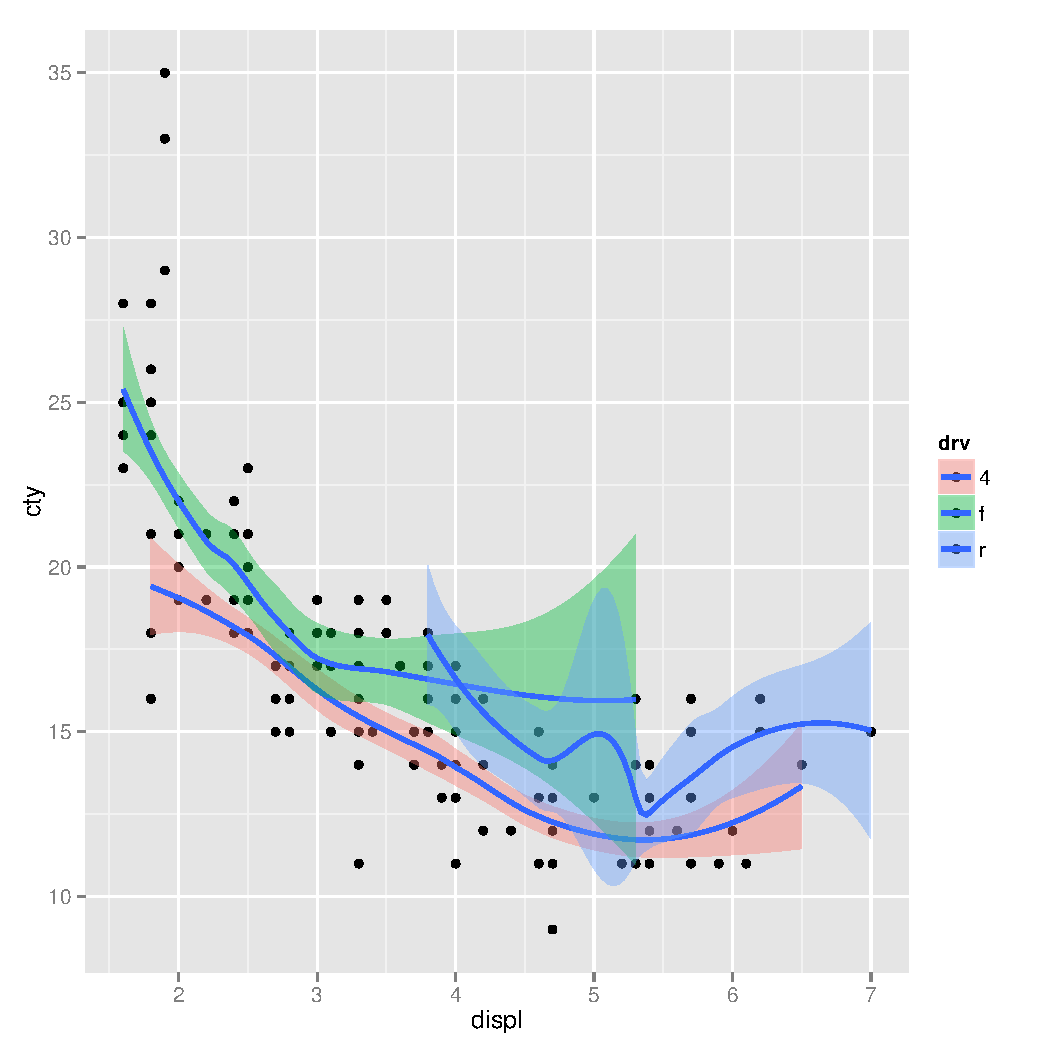
\includegraphics[width=\maxwidth]{figure/plot02-1} \caption[Figure 2]{Figure 2: City miles per gallon as a function of engine displacement for 4-wheele drive (4), front-wheel drive (f) and rear-wheel drive (r) cars.}\label{fig:plot02}
\end{figure}


\end{knitrout}

Four-wheel-drived cars are less ecomomical per miles





\end{document}
